% !TEX root = ../report.tex

\section{High level application description}

\subsection{Description}
Tinfnity is a mobile application that implements a proximity chat system aiming to connect people in the same area. In order to access this application, the user must connect his Facebook account and share some of his informations like photos and interests. This step, simplifies the login process and mitigates the fake users problem delegating the issue to Facebook. Once the user has been successfully logged in the application, he can discover all the people that are using Tinfinity near to him using the map as shown in Figure 1. If the user finds someone interesting on the map, he can tap on the marker and send a friendship request as shown in Figure 2.

\begin{multicols}{2}
\begin{figure}[H]
\centering
\centering
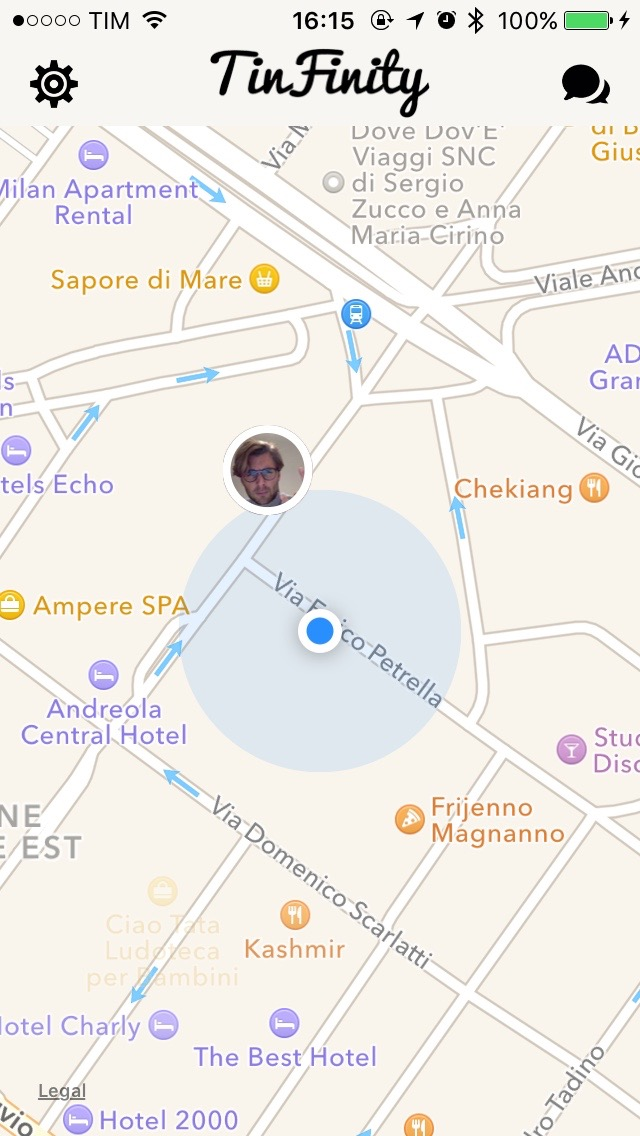
\includegraphics[scale=0.15]{./images/map.jpg}
\caption{\label{Users Map}Users Map}
\end{figure}

\begin{figure}[H]
\centering
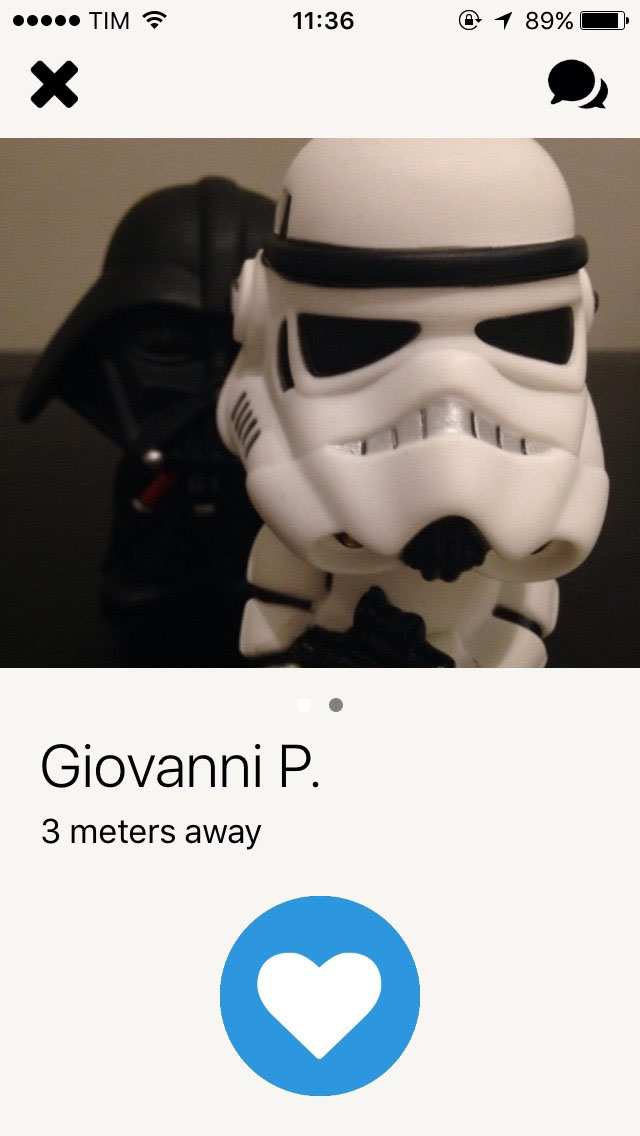
\includegraphics[scale=0.15]{./images/friendship_req.jpg}
\caption{\label{Friendship request}Friendship request}
\end{figure}
\end{multicols}

When and if recipient accepts the request, as shown in Figure 3, they can start chatting and maybe know each other directly in person. Also, when the friendship is granted, the two users can continue to chat even if they are no longer near such a normal chat system as Whatsapp for example, shown in Figure 4.

\newpage

\begin{multicols}{2}
\begin{figure}[H]
\centering
\centering
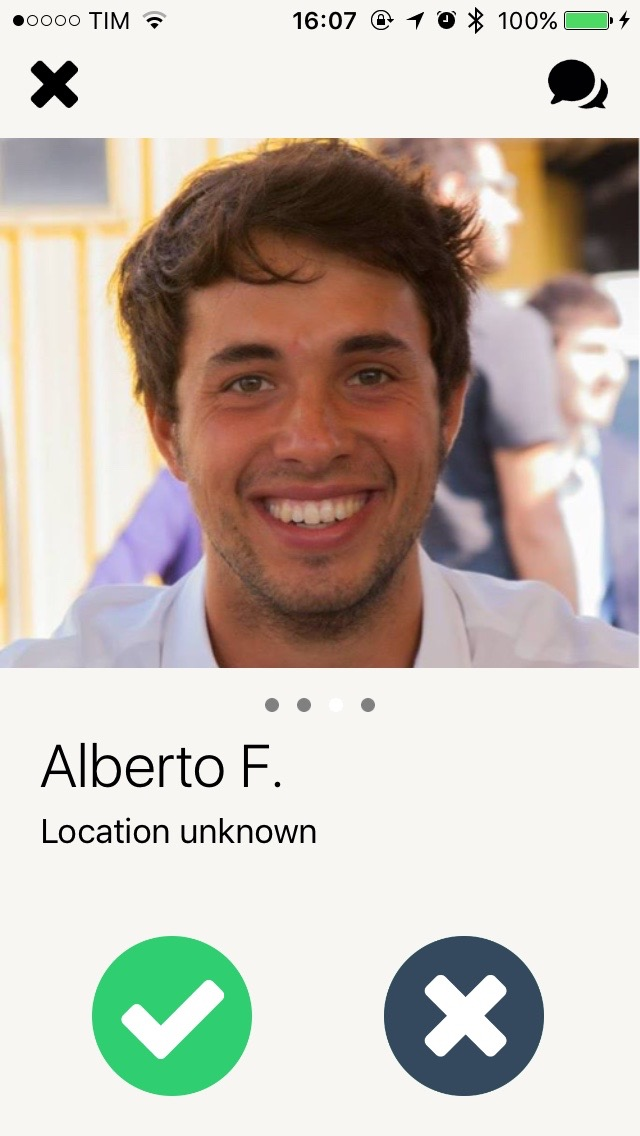
\includegraphics[scale=0.15]{./images/friendship_acc.jpg}
\caption{\label{Friendhip acceptance}Friendship acceptance}
\end{figure}

\begin{figure}[H]
\centering

\includegraphics[scale=0.15]{./images/chat.jpg}
\caption{\label{Chat}Chat}
\end{figure}
\end{multicols}

The user can also see the informations relative to his profile (Figure 5) and personalise which photos have to be shared with other through the settings page as shown in Figure 6.

\begin{multicols}{2}
\begin{figure}[H]
\centering
\centering
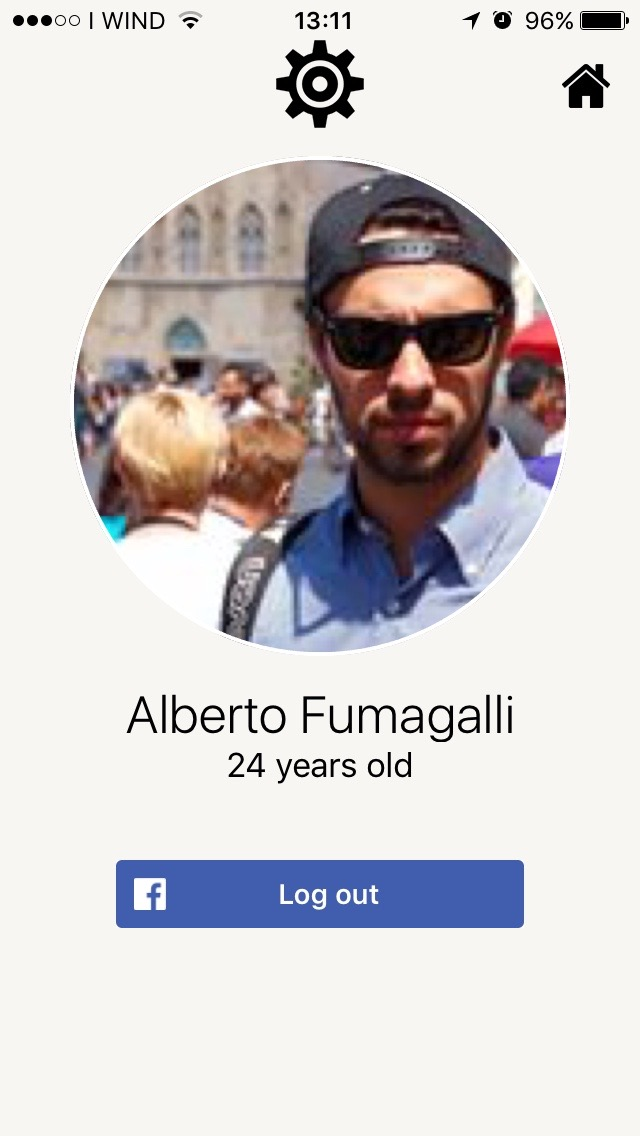
\includegraphics[scale=0.15]{./images/profile.jpg}
\caption{\label{Profile}Profile}
\end{figure}

\begin{figure}[H]
\centering
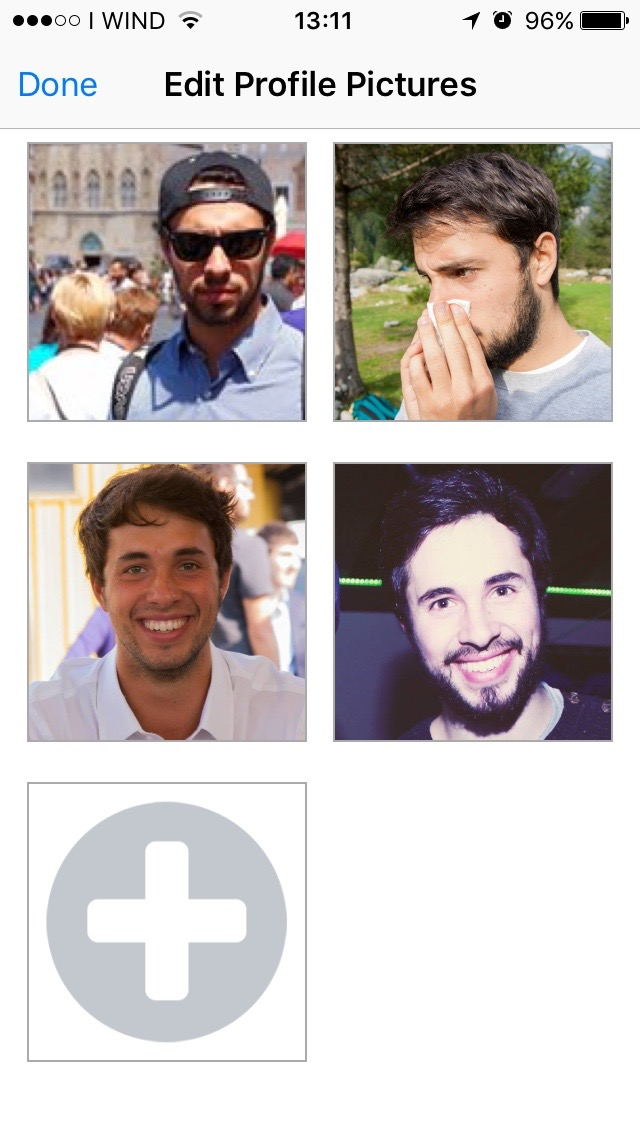
\includegraphics[scale=0.15]{./images/photo_selection.jpg}
\caption{\label{Profile}Profile}
\end{figure}
\end{multicols}

The application works in background and there is no need to open it in order to be localised by the others on the map.


